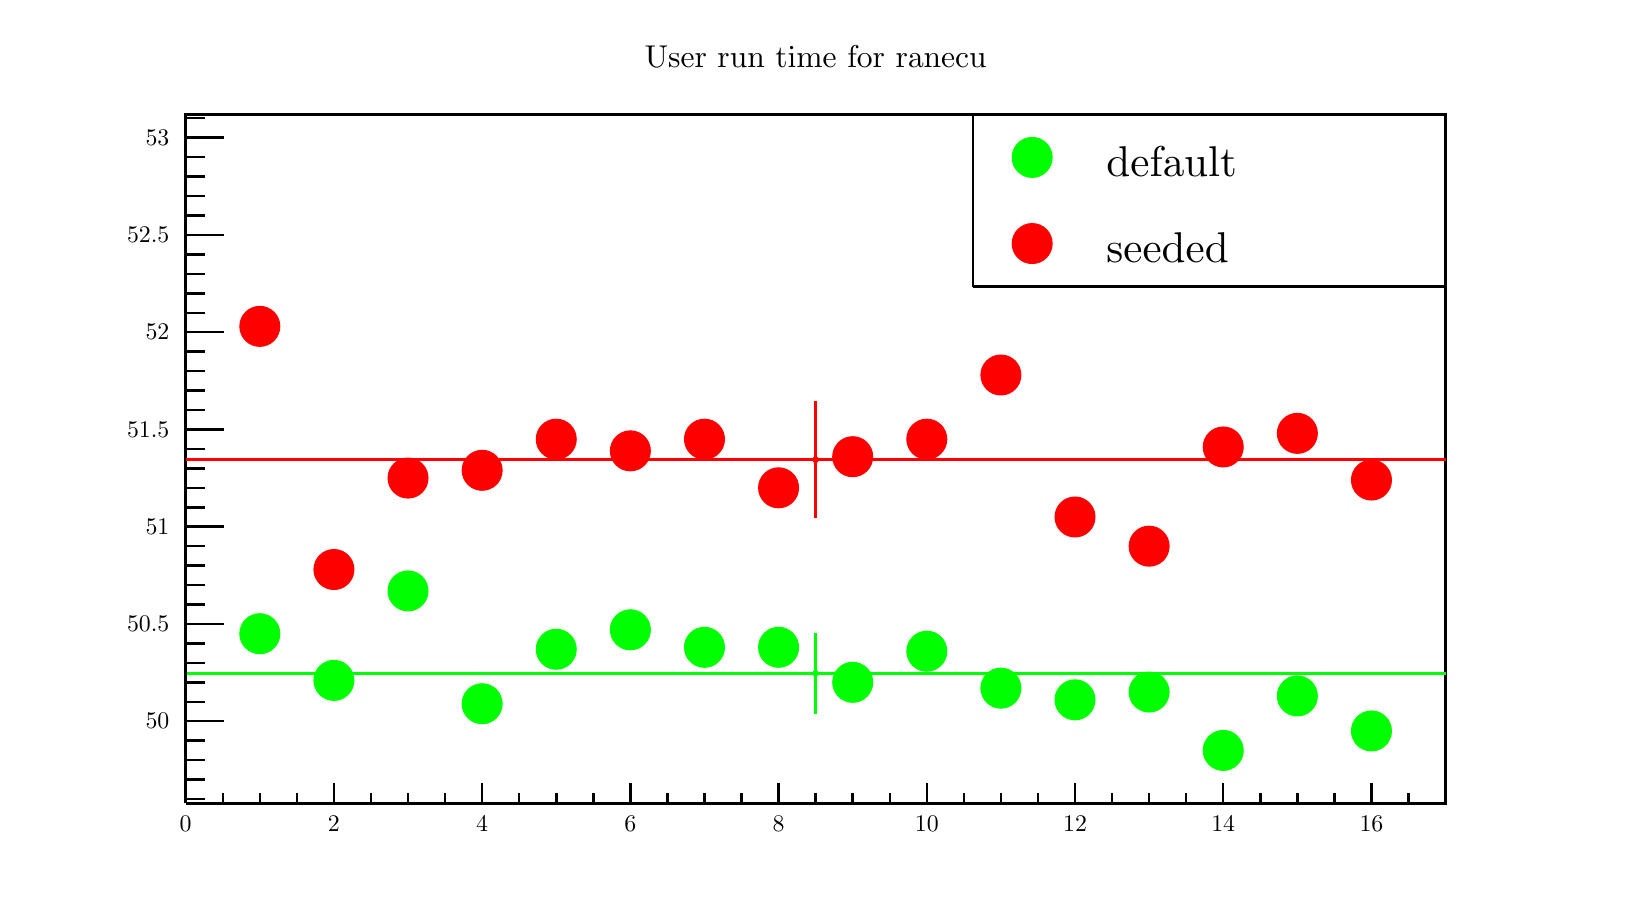
\begin{tikzpicture}
\pgfdeclareplotmark{cross} {
\pgfpathmoveto{\pgfpoint{-0.3\pgfplotmarksize}{\pgfplotmarksize}}
\pgfpathlineto{\pgfpoint{+0.3\pgfplotmarksize}{\pgfplotmarksize}}
\pgfpathlineto{\pgfpoint{+0.3\pgfplotmarksize}{0.3\pgfplotmarksize}}
\pgfpathlineto{\pgfpoint{+1\pgfplotmarksize}{0.3\pgfplotmarksize}}
\pgfpathlineto{\pgfpoint{+1\pgfplotmarksize}{-0.3\pgfplotmarksize}}
\pgfpathlineto{\pgfpoint{+0.3\pgfplotmarksize}{-0.3\pgfplotmarksize}}
\pgfpathlineto{\pgfpoint{+0.3\pgfplotmarksize}{-1.\pgfplotmarksize}}
\pgfpathlineto{\pgfpoint{-0.3\pgfplotmarksize}{-1.\pgfplotmarksize}}
\pgfpathlineto{\pgfpoint{-0.3\pgfplotmarksize}{-0.3\pgfplotmarksize}}
\pgfpathlineto{\pgfpoint{-1.\pgfplotmarksize}{-0.3\pgfplotmarksize}}
\pgfpathlineto{\pgfpoint{-1.\pgfplotmarksize}{0.3\pgfplotmarksize}}
\pgfpathlineto{\pgfpoint{-0.3\pgfplotmarksize}{0.3\pgfplotmarksize}}
\pgfpathclose
\pgfusepathqstroke
}
\pgfdeclareplotmark{cross*} {
\pgfpathmoveto{\pgfpoint{-0.3\pgfplotmarksize}{\pgfplotmarksize}}
\pgfpathlineto{\pgfpoint{+0.3\pgfplotmarksize}{\pgfplotmarksize}}
\pgfpathlineto{\pgfpoint{+0.3\pgfplotmarksize}{0.3\pgfplotmarksize}}
\pgfpathlineto{\pgfpoint{+1\pgfplotmarksize}{0.3\pgfplotmarksize}}
\pgfpathlineto{\pgfpoint{+1\pgfplotmarksize}{-0.3\pgfplotmarksize}}
\pgfpathlineto{\pgfpoint{+0.3\pgfplotmarksize}{-0.3\pgfplotmarksize}}
\pgfpathlineto{\pgfpoint{+0.3\pgfplotmarksize}{-1.\pgfplotmarksize}}
\pgfpathlineto{\pgfpoint{-0.3\pgfplotmarksize}{-1.\pgfplotmarksize}}
\pgfpathlineto{\pgfpoint{-0.3\pgfplotmarksize}{-0.3\pgfplotmarksize}}
\pgfpathlineto{\pgfpoint{-1.\pgfplotmarksize}{-0.3\pgfplotmarksize}}
\pgfpathlineto{\pgfpoint{-1.\pgfplotmarksize}{0.3\pgfplotmarksize}}
\pgfpathlineto{\pgfpoint{-0.3\pgfplotmarksize}{0.3\pgfplotmarksize}}
\pgfpathclose
\pgfusepathqfillstroke
}
\pgfdeclareplotmark{newstar} {
\pgfpathmoveto{\pgfqpoint{0pt}{\pgfplotmarksize}}
\pgfpathlineto{\pgfqpointpolar{44}{0.5\pgfplotmarksize}}
\pgfpathlineto{\pgfqpointpolar{18}{\pgfplotmarksize}}
\pgfpathlineto{\pgfqpointpolar{-20}{0.5\pgfplotmarksize}}
\pgfpathlineto{\pgfqpointpolar{-54}{\pgfplotmarksize}}
\pgfpathlineto{\pgfqpointpolar{-90}{0.5\pgfplotmarksize}}
\pgfpathlineto{\pgfqpointpolar{234}{\pgfplotmarksize}}
\pgfpathlineto{\pgfqpointpolar{198}{0.5\pgfplotmarksize}}
\pgfpathlineto{\pgfqpointpolar{162}{\pgfplotmarksize}}
\pgfpathlineto{\pgfqpointpolar{134}{0.5\pgfplotmarksize}}
\pgfpathclose
\pgfusepathqstroke
}
\pgfdeclareplotmark{newstar*} {
\pgfpathmoveto{\pgfqpoint{0pt}{\pgfplotmarksize}}
\pgfpathlineto{\pgfqpointpolar{44}{0.5\pgfplotmarksize}}
\pgfpathlineto{\pgfqpointpolar{18}{\pgfplotmarksize}}
\pgfpathlineto{\pgfqpointpolar{-20}{0.5\pgfplotmarksize}}
\pgfpathlineto{\pgfqpointpolar{-54}{\pgfplotmarksize}}
\pgfpathlineto{\pgfqpointpolar{-90}{0.5\pgfplotmarksize}}
\pgfpathlineto{\pgfqpointpolar{234}{\pgfplotmarksize}}
\pgfpathlineto{\pgfqpointpolar{198}{0.5\pgfplotmarksize}}
\pgfpathlineto{\pgfqpointpolar{162}{\pgfplotmarksize}}
\pgfpathlineto{\pgfqpointpolar{134}{0.5\pgfplotmarksize}}
\pgfpathclose
\pgfusepathqfillstroke
}
\definecolor{c}{rgb}{1,1,1};
\draw [color=c, fill=c] (0,0) rectangle (20,10.9387);
\draw [color=c, fill=c] (2,1.09387) rectangle (18,9.84481);
\definecolor{c}{rgb}{0,0,0};
\draw [c,line width=0.9] (2,1.09387) -- (2,9.84481) -- (18,9.84481) -- (18,1.09387) -- (2,1.09387);
\definecolor{c}{rgb}{1,1,1};
\draw [color=c, fill=c] (2,1.09387) rectangle (18,9.84481);
\definecolor{c}{rgb}{0,0,0};
\draw [c,line width=0.9] (2,1.09387) -- (2,9.84481) -- (18,9.84481) -- (18,1.09387) -- (2,1.09387);
\definecolor{c}{rgb}{0,1,0};
\draw [c,line width=0.9] (10,2.22967) -- (10,2.74586);
\draw [c,line width=0.9] (10,2.74586) -- (10,3.26205);
\draw [c,line width=0.9] (2,2.74586) -- (10,2.74586);
\draw [c,line width=0.9] (10,2.74586) -- (18,2.74586);
\foreach \P in {(10,2.74586)}{\draw[mark options={color=c,fill=c},mark size=2.402402pt,mark=*,mark size=1pt] plot coordinates {\P};}
\definecolor{c}{rgb}{0,0,0};
\draw [c,line width=0.9] (2,1.09387) -- (18,1.09387);
\draw [c,line width=0.9] (2,1.3564) -- (2,1.09387);
\draw [c,line width=0.9] (2.47059,1.22513) -- (2.47059,1.09387);
\draw [c,line width=0.9] (2.94118,1.22513) -- (2.94118,1.09387);
\draw [c,line width=0.9] (3.41176,1.22513) -- (3.41176,1.09387);
\draw [c,line width=0.9] (3.88235,1.3564) -- (3.88235,1.09387);
\draw [c,line width=0.9] (4.35294,1.22513) -- (4.35294,1.09387);
\draw [c,line width=0.9] (4.82353,1.22513) -- (4.82353,1.09387);
\draw [c,line width=0.9] (5.29412,1.22513) -- (5.29412,1.09387);
\draw [c,line width=0.9] (5.76471,1.3564) -- (5.76471,1.09387);
\draw [c,line width=0.9] (6.23529,1.22513) -- (6.23529,1.09387);
\draw [c,line width=0.9] (6.70588,1.22513) -- (6.70588,1.09387);
\draw [c,line width=0.9] (7.17647,1.22513) -- (7.17647,1.09387);
\draw [c,line width=0.9] (7.64706,1.3564) -- (7.64706,1.09387);
\draw [c,line width=0.9] (8.11765,1.22513) -- (8.11765,1.09387);
\draw [c,line width=0.9] (8.58823,1.22513) -- (8.58823,1.09387);
\draw [c,line width=0.9] (9.05882,1.22513) -- (9.05882,1.09387);
\draw [c,line width=0.9] (9.52941,1.3564) -- (9.52941,1.09387);
\draw [c,line width=0.9] (10,1.22513) -- (10,1.09387);
\draw [c,line width=0.9] (10.4706,1.22513) -- (10.4706,1.09387);
\draw [c,line width=0.9] (10.9412,1.22513) -- (10.9412,1.09387);
\draw [c,line width=0.9] (11.4118,1.3564) -- (11.4118,1.09387);
\draw [c,line width=0.9] (11.8824,1.22513) -- (11.8824,1.09387);
\draw [c,line width=0.9] (12.3529,1.22513) -- (12.3529,1.09387);
\draw [c,line width=0.9] (12.8235,1.22513) -- (12.8235,1.09387);
\draw [c,line width=0.9] (13.2941,1.3564) -- (13.2941,1.09387);
\draw [c,line width=0.9] (13.7647,1.22513) -- (13.7647,1.09387);
\draw [c,line width=0.9] (14.2353,1.22513) -- (14.2353,1.09387);
\draw [c,line width=0.9] (14.7059,1.22513) -- (14.7059,1.09387);
\draw [c,line width=0.9] (15.1765,1.3564) -- (15.1765,1.09387);
\draw [c,line width=0.9] (15.6471,1.22513) -- (15.6471,1.09387);
\draw [c,line width=0.9] (16.1176,1.22513) -- (16.1176,1.09387);
\draw [c,line width=0.9] (16.5882,1.22513) -- (16.5882,1.09387);
\draw [c,line width=0.9] (17.0588,1.3564) -- (17.0588,1.09387);
\draw [c,line width=0.9] (17.0588,1.3564) -- (17.0588,1.09387);
\draw [c,line width=0.9] (17.5294,1.22513) -- (17.5294,1.09387);
\draw [c,line width=0.9] (18,1.22513) -- (18,1.09387);
\draw [anchor=base] (2,0.732891) node[scale=0.861703, color=c, rotate=0]{0};
\draw [anchor=base] (3.88235,0.732891) node[scale=0.861703, color=c, rotate=0]{2};
\draw [anchor=base] (5.76471,0.732891) node[scale=0.861703, color=c, rotate=0]{4};
\draw [anchor=base] (7.64706,0.732891) node[scale=0.861703, color=c, rotate=0]{6};
\draw [anchor=base] (9.52941,0.732891) node[scale=0.861703, color=c, rotate=0]{8};
\draw [anchor=base] (11.4118,0.732891) node[scale=0.861703, color=c, rotate=0]{10};
\draw [anchor=base] (13.2941,0.732891) node[scale=0.861703, color=c, rotate=0]{12};
\draw [anchor=base] (15.1765,0.732891) node[scale=0.861703, color=c, rotate=0]{14};
\draw [anchor=base] (17.0588,0.732891) node[scale=0.861703, color=c, rotate=0]{16};
\draw [c,line width=0.9] (2,1.09387) -- (2,9.84481);
\draw [c,line width=0.9] (2.48,2.13756) -- (2,2.13756);
\draw [c,line width=0.9] (2.24,2.38458) -- (2,2.38458);
\draw [c,line width=0.9] (2.24,2.63161) -- (2,2.63161);
\draw [c,line width=0.9] (2.24,2.87864) -- (2,2.87864);
\draw [c,line width=0.9] (2.24,3.12567) -- (2,3.12567);
\draw [c,line width=0.9] (2.48,3.37269) -- (2,3.37269);
\draw [c,line width=0.9] (2.24,3.61972) -- (2,3.61972);
\draw [c,line width=0.9] (2.24,3.86675) -- (2,3.86675);
\draw [c,line width=0.9] (2.24,4.11377) -- (2,4.11377);
\draw [c,line width=0.9] (2.24,4.3608) -- (2,4.3608);
\draw [c,line width=0.9] (2.48,4.60783) -- (2,4.60783);
\draw [c,line width=0.9] (2.24,4.85486) -- (2,4.85486);
\draw [c,line width=0.9] (2.24,5.10188) -- (2,5.10188);
\draw [c,line width=0.9] (2.24,5.34891) -- (2,5.34891);
\draw [c,line width=0.9] (2.24,5.59594) -- (2,5.59594);
\draw [c,line width=0.9] (2.48,5.84297) -- (2,5.84297);
\draw [c,line width=0.9] (2.24,6.08999) -- (2,6.08999);
\draw [c,line width=0.9] (2.24,6.33702) -- (2,6.33702);
\draw [c,line width=0.9] (2.24,6.58405) -- (2,6.58405);
\draw [c,line width=0.9] (2.24,6.83107) -- (2,6.83107);
\draw [c,line width=0.9] (2.48,7.0781) -- (2,7.0781);
\draw [c,line width=0.9] (2.24,7.32513) -- (2,7.32513);
\draw [c,line width=0.9] (2.24,7.57216) -- (2,7.57216);
\draw [c,line width=0.9] (2.24,7.81918) -- (2,7.81918);
\draw [c,line width=0.9] (2.24,8.06621) -- (2,8.06621);
\draw [c,line width=0.9] (2.48,8.31324) -- (2,8.31324);
\draw [c,line width=0.9] (2.24,8.56026) -- (2,8.56026);
\draw [c,line width=0.9] (2.24,8.80729) -- (2,8.80729);
\draw [c,line width=0.9] (2.24,9.05432) -- (2,9.05432);
\draw [c,line width=0.9] (2.24,9.30135) -- (2,9.30135);
\draw [c,line width=0.9] (2.48,9.54837) -- (2,9.54837);
\draw [c,line width=0.9] (2.48,2.13756) -- (2,2.13756);
\draw [c,line width=0.9] (2.24,1.89053) -- (2,1.89053);
\draw [c,line width=0.9] (2.24,1.6435) -- (2,1.6435);
\draw [c,line width=0.9] (2.24,1.39648) -- (2,1.39648);
\draw [c,line width=0.9] (2.24,1.14945) -- (2,1.14945);
\draw [c,line width=0.9] (2.48,9.54837) -- (2,9.54837);
\draw [c,line width=0.9] (2.24,9.7954) -- (2,9.7954);
\draw [anchor= east] (1.9,2.13756) node[scale=0.861703, color=c, rotate=0]{50};
\draw [anchor= east] (1.9,3.37269) node[scale=0.861703, color=c, rotate=0]{50.5};
\draw [anchor= east] (1.9,4.60783) node[scale=0.861703, color=c, rotate=0]{51};
\draw [anchor= east] (1.9,5.84297) node[scale=0.861703, color=c, rotate=0]{51.5};
\draw [anchor= east] (1.9,7.0781) node[scale=0.861703, color=c, rotate=0]{52};
\draw [anchor= east] (1.9,8.31324) node[scale=0.861703, color=c, rotate=0]{52.5};
\draw [anchor= east] (1.9,9.54837) node[scale=0.861703, color=c, rotate=0]{53};
\definecolor{c}{rgb}{1,0,0};
\draw [c,line width=0.9] (10,4.71345) -- (10,5.45853);
\draw [c,line width=0.9] (10,5.45853) -- (10,6.20361);
\draw [c,line width=0.9] (2,5.45853) -- (10,5.45853);
\draw [c,line width=0.9] (10,5.45853) -- (18,5.45853);
\foreach \P in {(10,5.45853)}{\draw[mark options={color=c,fill=c},mark size=2.402402pt,mark=*,mark size=1pt] plot coordinates {\P};}
\definecolor{c}{rgb}{0,1,0};
\foreach \P in {(2.94118,3.24918), (3.88235,2.65631), (4.82353,3.79264), (5.76471,2.35988), (6.70588,3.05156), (7.64706,3.29859), (8.58823,3.07626), (9.52941,3.07626), (10.4706,2.63161), (11.4118,3.02686), (12.3529,2.5575), (13.2941,2.40929),
 (14.2353,2.5081), (15.1765,1.76702), (16.1176,2.45869), (17.0588,2.01404)}{\draw[mark options={color=c,fill=c},mark size=7.207207pt,mark=*] plot coordinates {\P};}
\definecolor{c}{rgb}{1,0,0};
\foreach \P in {(2.94118,7.15221), (3.88235,4.06437), (4.82353,5.2254), (5.76471,5.32421), (6.70588,5.71945), (7.64706,5.57124), (8.58823,5.71945), (9.52941,5.10188), (10.4706,5.49713), (11.4118,5.71945), (12.3529,6.53464), (13.2941,4.73134),
 (14.2353,4.3608), (15.1765,5.62064), (16.1176,5.79356), (17.0588,5.20069)}{\draw[mark options={color=c,fill=c},mark size=7.207207pt,mark=*] plot coordinates {\P};}
\definecolor{c}{rgb}{1,1,1};
\draw [color=c, fill=c] (12,7.65707) rectangle (18,9.84481);
\definecolor{c}{rgb}{0,0,0};
\draw [c,line width=0.9] (12,7.65707) -- (18,7.65707);
\draw [c,line width=0.9] (18,7.65707) -- (18,9.84481);
\draw [c,line width=0.9] (18,9.84481) -- (12,9.84481);
\draw [c,line width=0.9] (12,9.84481) -- (12,7.65707);
\draw [anchor=base west] (13.5,9.05175) node[scale=1.55662, color=c, rotate=0]{default};
\definecolor{c}{rgb}{1,1,1};
\draw [c] (12.225,8.91502) -- (13.275,8.91502) -- (13.275,9.68073) -- (12.225,9.68073);
\draw [c,line width=0.9] (12.225,9.29787) -- (13.275,9.29787);
\definecolor{c}{rgb}{0,1,0};
\foreach \P in {(12.75,9.29787)}{\draw[mark options={color=c,fill=c},mark size=7.207207pt,mark=*] plot coordinates {\P};}
\definecolor{c}{rgb}{0,0,0};
\draw [anchor=base west] (13.5,7.95788) node[scale=1.55662, color=c, rotate=0]{seeded};
\definecolor{c}{rgb}{1,1,1};
\draw [c] (12.225,7.82115) -- (13.275,7.82115) -- (13.275,8.58686) -- (12.225,8.58686);
\draw [c,line width=0.9] (12.225,8.20401) -- (13.275,8.20401);
\definecolor{c}{rgb}{1,0,0};
\foreach \P in {(12.75,8.20401)}{\draw[mark options={color=c,fill=c},mark size=7.207207pt,mark=*] plot coordinates {\P};}
\definecolor{c}{rgb}{0,0,0};
\draw (10,10.5832) node[scale=1.13967, color=c, rotate=0]{User run time for ranecu};
\end{tikzpicture}
